%%% IMPORTANT: COMPILE WITH XeLaTeX

\documentclass[12pt]{article}
%All packages used this far
%\usepackage[latin1]{inputenc}
%\usepackage{times}
%\usepackage{logicproof}
%\usepackage{enumerate}
%\usepackage{cancel}
\usepackage{fullpage} % required for this template
%\usepackage{color}
%\usepackage{qtree}
%\usepackage{amsmath}
\usepackage{fontspec} % required for this template
%\usepackage{amssymb}
%\usepackage{amsthm}
%\usepackage{prooftrees}
\usepackage{tikz}
%\usepackage{circuitikz}
%\usepackage{colortbl}
%\usepackage{karnaugh-map}
%\usepackage[margin=1in]{geometry} % not sure if useful
%\usepackage{indentfirst}
%\usepackage{pgfplots}
%\usepackage{xcolor}
%\usepackage{arydshln}
%\usepackage{hyperref}

% Tikz libraries
%\usetikzlibrary{positioning}
%\usetikzlibrary{shapes.multipart}
%\usetikzlibrary{decorations.text}
%\usetikzlibrary{datavisualization}
%\usetikzlibrary{datavisualization.formats.functions}
%\usetikzlibrary{patterns}
%\usetikzlibrary{arrows.meta}
%\usetikzlibrary{quotes}
%\usetikzlibrary{automata}


\setromanfont{Times New Roman}
\setsansfont{Helvetica}

%Symbols that might be necessary
%\DeclareMathSymbol{@}{\mathord}{letters}{"3B}
%\newcommand{\powerset}{\raisebox{.15\baselineskip}{\Large\ensuremath{\wp}}}

\begin{document}

\noindent
Universidade Federal do Rio Grande do Sul \hfill Instituto de Informática \newline 
INF01009 -- Computação Gráfica \hfill 2023/1 \newline
Aluno \hfill Pedro Company Beck -- 00324055
\rule{\linewidth}{1.pt}

\begin{center}
	\LARGE\textbf{Assignment 0} 
\end{center}

The provided source files compiled with no issues using make with the MinGW compiler on Windows 7, as shown below:
\begin{center}
	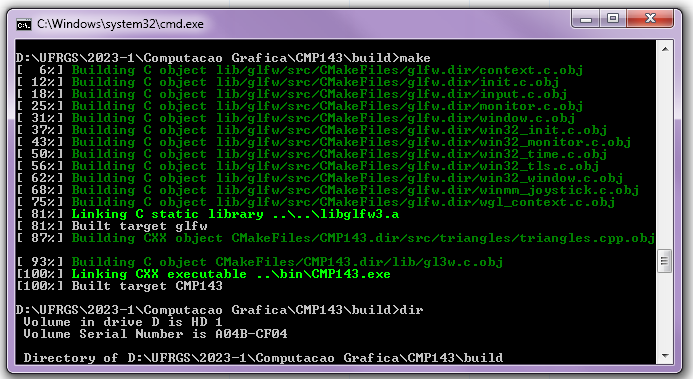
\includegraphics[scale=0.5]{1.png}
\end{center}
And the result without modifying the source files was the following:
\begin{center}
	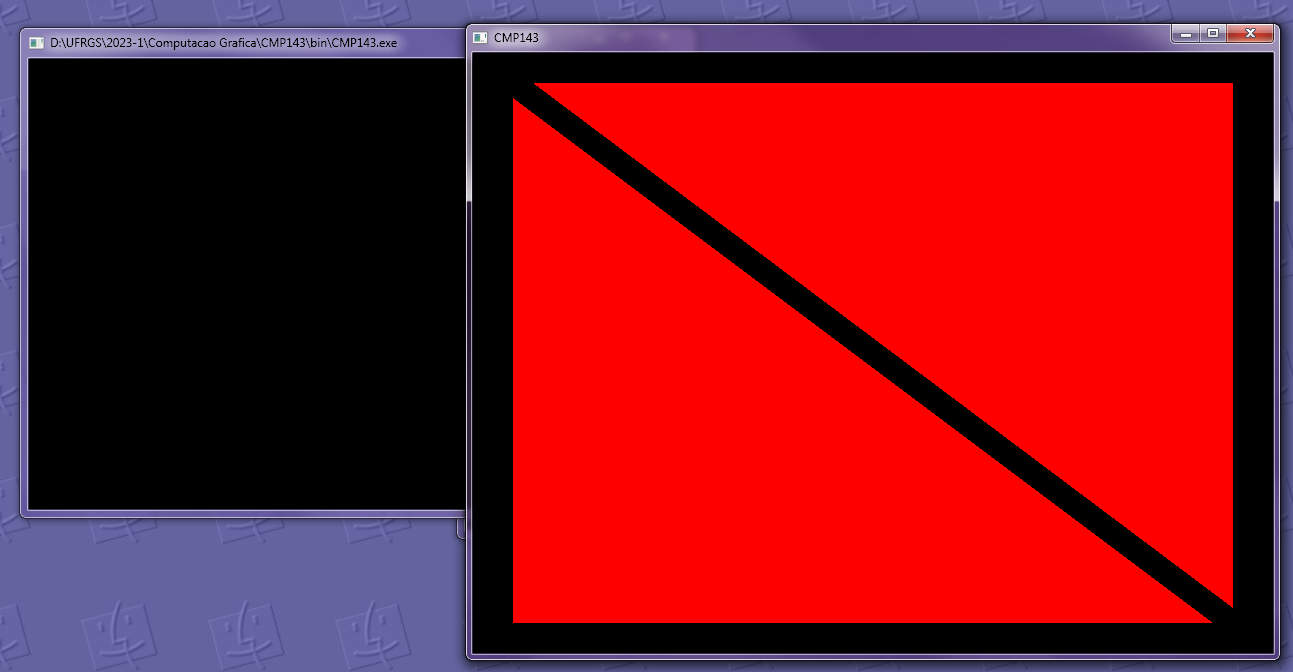
\includegraphics[scale=0.5]{2.png}
\end{center}
After modifying the \texttt{triangles.cpp} file to show only one triangle, using the colors red, green, and blue for the vertices of the triangle, the result obtained was the following:
\begin{center}
	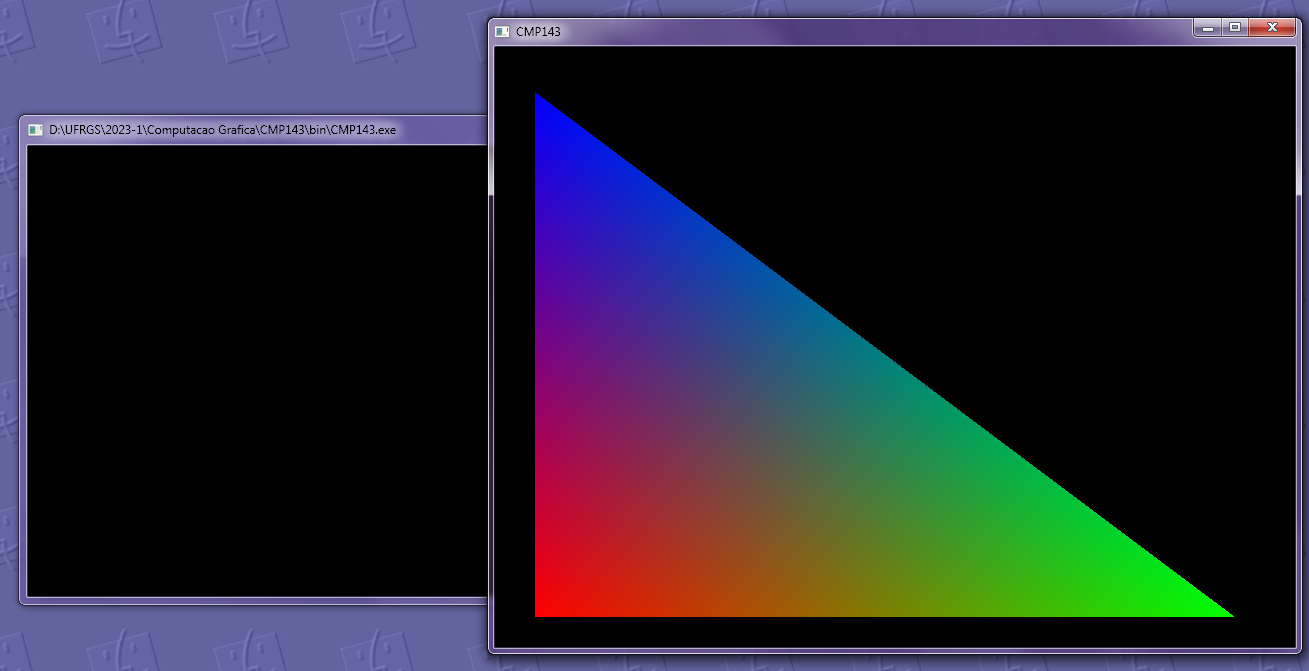
\includegraphics[scale=0.5]{4.png}
\end{center}
The modified source code is included with this report.


\end{document}